\documentclass[oneside,14pt,a4paper]{extreport}

% LANGUAGE
\usepackage[T2A]{fontenc}
\usepackage[utf8]{inputenc}
\usepackage[english, ukrainian]{babel}

% \usepackage{minted}
\usepackage{pgfplots}

% VARIABLES
\newcommand \labno    {4}
\newcommand \course   {Науковий процес та робота з науковими джерелами}
\newcommand \group    {409}
\newcommand \lecturer {Ізонін І. В.}
\newcommand \theme    {Основи етики наукових досліджень: плагіат та засоби його виявлення}
\newcommand \purpose  {Ознайомитися із поняттям \flqq{}академічної доброчесності\frqq{}, навчитися здійснювати перевірку тексту на ункікальність із використанням спеціалізованих засобів.}

% PACKAGES
\usepackage{amssymb}
\usepackage{amsmath}
\usepackage{multirow}
\usepackage{url}
\usepackage[unicode=true]{hyperref}
\usepackage{hanging}

% GEOMETRY
\usepackage{geometry}
\geometry{left   = 2.5cm}
\geometry{right  = 1cm}
\geometry{top    = 2cm}
\geometry{bottom = 2cm}
\renewcommand {\baselinestretch} {1.5}
\setlength\parindent{1cm}

% IMAGES
\usepackage{graphicx}
\usepackage{indentfirst}
\graphicspath{ {./imgs/} }
\usepackage{float}

% FOOTER
\usepackage{fancyhdr}
\fancyhf{}
\renewcommand{\headrulewidth}{0pt}
\cfoot{\hfill \thepage}
\pagestyle{fancy}

% CHAPTERS

\newcommand\Section[1]{
 \refstepcounter{section}
 \section*{
  \arabic{section}. #1}
}

\newcommand\Subsection[1]{
 \refstepcounter{subsection}
 \section*{
  \arabic{section}.\arabic{subsection}. #1}
}

\sloppy
\begin{document}
\begin{titlepage}

\centering
 \textbf{
  МІНІСТЕРСТВО ОСВІТИ І НАУКИ УКРАЇНИ \
  НАЦІОНАЛЬНИЙ УНІВЕРСИТЕТ \flqq{}ЛЬВІВСЬКА ПОЛІТЕХНІКА\frqq{} \
  ІНСТИТУТ КОМП’ЮТЕРНИХ НАУК ТА ІНФОРМАЦІЙНИХ ТЕХНОЛОГІЙ
 }

\vspace{0.5cm}
 \textbf{
  Кафедра систем штучного інтелекту
}

\vspace*{\fill}

  {
    \centering
    
\includegraphics[width=7cm]{imgs/logo.eps}
  }

\vspace{1cm}

  {\textbf{ЗВІТ} \par{}
  {про виконання практичної роботи №\labno}
   \par}
  {з курсу \flqq{}\course\frqq{} \par}

\vspace{1cm} \theme

\raggedleft\vfill

 {\textbf{Виконав:} \par}
 {ст. гр. КН-\group \par}
 {Тимошенко Павло Олександрович \par}

% \vspace{1cm}

 {\textbf{Перевірив:} \par}
 {доцент каф. СШІ, к.т.н.,}
 {\lecturer \par}

\vspace{1cm}

\centering {Львів -- \the\year \par}

\end{titlepage}

\Section{Постановка завдання}

Далі описано пункти, які потрібно виконати у межах цієї практичної роботи.

\begin{enumerate}
    \item Ознайомитись із поняттям \flqq{}академічної доброчесності\frqq{} та видами академічного плагіату.
    \item Здійснити перевірку звіту до практикти (1 сторінки тексту) із використанням двох довільних програм сервісів. Подати результати перевірки, порівняти результати, отримані двома різними програмами.
    \item Описати основні шляхи уникнення плагіату. Подати основні кроки усунення елементів плагіату з аналізованої роботи.
    \item Здійснити опис проведеної роботи.
\end{enumerate}

\Section{Хід роботи}

В цьому розділі описано процес виконання практичної роботи та пророблені кроки. 

Я не зміг знайти свій звіт з практичної роботи у швидкому доступі, тому у цій практичній роботі аналізував уривок (розміром в одну сторінку) з розділу \flqq{}Обговорення результатів експериментів\frqq{} з курсової роботи.

\Subsection{Аналізований текст}

Такі результати, як 81\% точності при класифікації слів та 71\% точності при маркуванні речень, не можна вважати дуже високими. Втім, у цій роботі ми показово не використовували жодного препроцесингу чи виправлення результатів -- це зроблено для демонстрації того, що розглянуті алгоритми є потужними та надійними навіть на сирих необроблених даних. Імплементація та аналіз різних технік покращення результату виходять за межі задач, поставлених на початку роботи. Однак, найдієвіші з них все одно варто згадати, оскільки це може мати цінність для подальших досліджень:

\begin{itemize}
    \item для частин мови, склад яких не має тенденції змінюватись з часом (службові частини мови та займенники), можна створити список. Тепер слова, які входитимуть у такі списки можна класифікувати із стовідсотковою точністю;
    \item при тренуванні моделі ПММ замість того, щоби додавати у матрицю ймовірностей спостережень кожне слово із частиною мови що згадані вище, можна додати спеціальний об'єкт, який позначатиме всю частину мови в цілому. Завдяки цьому зменшиться кількість об'єктів, що зберігаються у моделі, а отже і розмір у пам'яті та час класифікації;
    \item мітки \texttt{X}, \texttt{PUNCT} та \texttt{SYM}, що відповідають за іноземні слова (або просто випадкових набір символів), пунктуацію та будь-які інші небуквенні символи відповідно можна визначати алгоритмічно;
    \item у промаркованому реченні можна визначати стійкі помилкові патерни та виправляти їх. Такий підхід також відомий як \flqq{}маркувальник Бриля\frqq{}.
\end{itemize}

Окремої уваги заслуговують результати експерименту із прорідженням простору. Їх можна розуміти так, що існує спосіб скоротити обсяг тренувальних даних для задачі класифікації, але при цьому не зменшити точність отриманої моделі. [...]

\Section{Перевірка сервісом Content-watch}

Для того, аби перевірити текст, написаний у Latex-форматі за допомогою сервісу Content-watch\cite{content-watch}, я видалив із нього все форматування та вставив у поле тексту, як показано на Рис.~\ref{pic:content-watch}. Результат цієї перевірки продемонстровано на Рис.~\ref{pic:result-content-watch}

\begin{figure}[H]
    \centering
    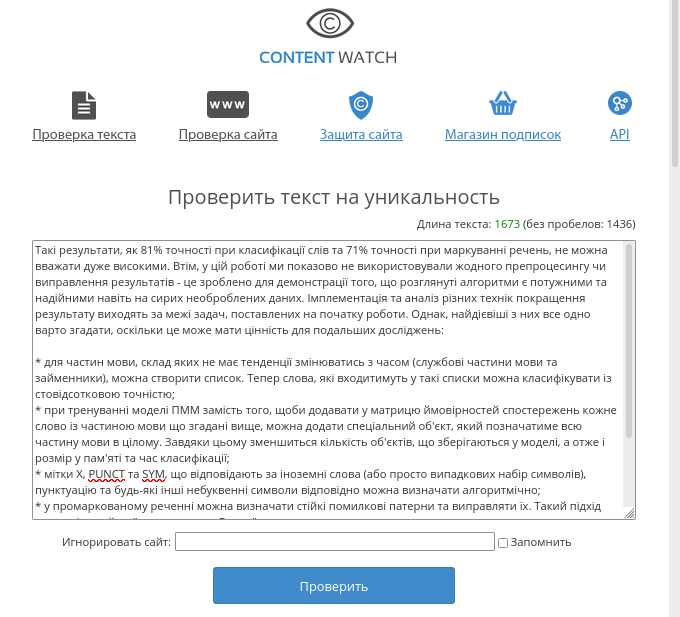
\includegraphics[width=.9\textwidth]{imgs/sp5-content-watch.png}
    \caption{Перевірка тексту на плагіат з використанням сервісу Content-watch.}
    \label{pic:content-watch}
\end{figure}

\begin{figure}[H]
    \centering
    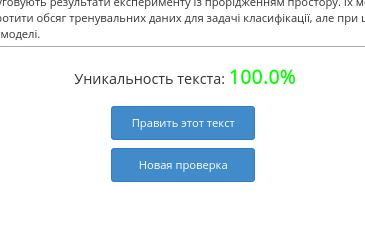
\includegraphics[width=.5\textwidth]{imgs/sp5-result-content-watch.png}
    \caption{Результат перевірки тексту сервісом Content-watch.}
    \label{pic:result-content-watch}
\end{figure}

\Section{Перевірка сервісом Etxt.ru}

Використовуючи сервіс etxt.ru\cite{etxt}, я виконав аналогічні дії. Процес перевірки та результат показано на Рис.~\ref{pic:etxt-ru} та Рис.~\ref{pic:result-etxt} відповідно.

\begin{figure}[H]
    \centering
    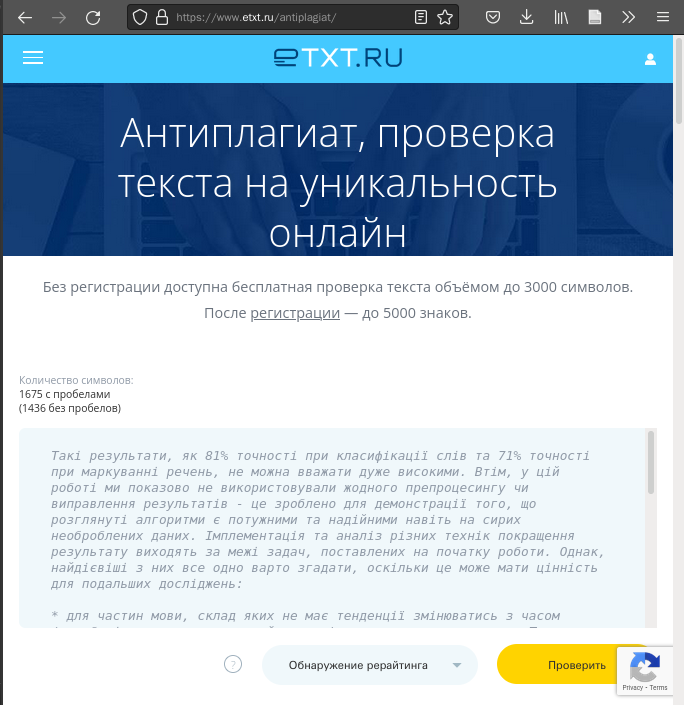
\includegraphics[width=.9\textwidth]{imgs/sp5-etxt-ru.png}
    \caption{Перевірка тексту на плагіат з використанням сервісу etxt.ru.}
    \label{pic:etxt-ru}
\end{figure}

\begin{figure}[H]
    \centering
    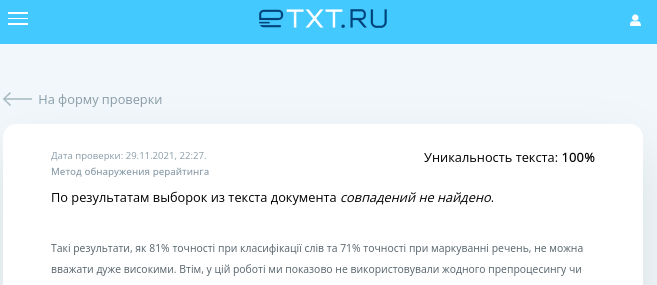
\includegraphics[width=.8\textwidth]{imgs/sp5-result-etxt.png}
    \caption{Результат перевірки тексту сервісом etxt.ru.}
    \label{pic:result-etxt}
\end{figure}

\Section{Результати та висновки}

Обидва сервіси показали, що мій текст має 100-відсоткову унікальність. Такий результат був неочікуваним, втім, я ним задоволений!

Це не обов'язково означає, що ніде у світі не існує більше роботи, вислови у якій, є схожими на мої. Цілком ймовірно, що подібні праці просто відсутні в базі пошуку абощо. При перевірці всього обсягу роботи ми навряд досягнемо 100-відсоткової унікальності, тому що навіть усталені вирази та схожі висновки (особливо коли текст не несе змістового навантаження, а є лише \flqq{}водою\frqq{}) можна вважати плагіатом. Тож для того, аби уникнути можливого плагіату, я сформулював для себе деякі принципи, які також міг би порадити і комусь іншому.

\begin{enumerate}
    \item Перш за все потрібно користуватись здоровим глуздом. Якщо адекватно і свідомо описувати результати власної роботи, з власними висновками та міркуваннями, то вірогідність того, що хтось уже використав такі самі висловлювання, на мою думку, є дуже малою.
    \item Потрібно уникати сталих беззмістовних виразів та тексту-\flqq{}води\frqq{}. Наприклад: \textit{у цій роботі ми здійснювали дослідження на предмет відповідності досліджуваного об'єкта очікуваним властивостям, сформульованим у меті}.
    \item При огляді літератури потрібно занотовувати цікаві думки, аби за потреби процитувати їх із правильним вказанням джерела. В іншому разі це може бути плагіатом.
\end{enumerate}

Досвід, отриманий в результаті виконання цієї роботи, я зможу використати при написанні диплому задля уникнення помилкового плагіату.

\Section{Список використаної літератури}

\begingroup
\renewcommand{\section}[2]{}
\renewcommand{\chapter}[2]{}
\begin{thebibliography}{99}

\bibitem{content-watch} Антиплагиат онлайн - проверить текст на уникальность без регистрации [Електронний ресурс] // Защита контента сайта от копирования. – Режим доступу: \url{https://content-watch.ru/text/} (дата звернення: 29.11.2021). – Назва з екрана.

\bibitem{etxt} Антиплагиат, проверить текст на уникальность онлайн. [Електронний ресурс] // Биржа копирайтинга eTXT. – Режим доступу: \url{https://www.etxt.ru/antiplagiat/} (дата звернення: 29.11.2021). – Назва з екрана.

\end{thebibliography}

\end{document}
